% Template for ISBI-2017 paper; to be used with:
%          spconf.sty  - ICASSP/ICIP LaTeX style file, and
%          IEEEbib.bst - IEEE bibliography style file.
% --------------------------------------------------------------------------
\documentclass{article}
%\usepackage[style=ieee,maxbibnames=9,maxcitenames=2,backend=biber]{biblatex}
\usepackage{spconf,amsmath,graphicx}
\usepackage{multirow}
\usepackage{gensymb}
\usepackage{amsmath}
\usepackage{booktabs}
\usepackage{subcaption}
\usepackage{flushend}

% Example definitions.
% --------------------
\def\x{{\mathbf x}}
\def\L{{\cal L}}


% Title.
% ------
\title{mesenchymal cell migration modes prediction in confocal microscopy images 
using bayesian deep learning}
%
% Single address.
% ---------------
\name{Anindya Gupta$^{1}$, 
Veronica Larsson$^{2}$, 
Nicolas Pielawski$^{1}$, 
Damian Matuszewski$^{1}$} 
\secondlinename{Staffan Strömblad$^{2}$, 
and Carolina Wählby$^{1}$}

 \address{$^{1}$ Centre for Image Analysis, Dept. 
 of Information Technology, Uppsala University, Sweden\\
     $^{2}$ Department of Biosciences and Nutrition, 
     Karolinska Institutet, Huddinge, Sweden\\}

\begin{document}
\maketitle
% Abstract-----------------------------------------------------
\begin{abstract}

Cell migration is a complex and heterogeneous phenomenon consisting of many spatially and
temporally regulated mechanisms. 
A complete understanding of cell migration phenomenon is indeed crucial to derive an 
adequate quantification for single cell-based analysis. 
However, the spatiotemporal behavior of dynamic cells is often complex and challenging for 
manual classification and analysis.\,Automatized algorithms are thus highly 
desired to facilitate mesenchymal migration sub-modalities prediction. 
Supervised deep learning techniques have shown promising outcomes in microscopy image 
analysis. However, their implication is confided by the amount of carefully annotated data.
Weak supervision provides a simple, model-agnostic way to integrate the domain-expertise   
into a learning model. 
Additionally, bayesian predicitons can lead to a more informed decision, and the quality 
of prediction can be improved.
% For comprehensive and adequate quantitative analysis, this work focuses on harnessing 
% the discriminative capabilities of deep learning based methods to perform real-time classification 
% of two migration modes, and thereafter, to increase the understanding of underlying phenomenon that 
% influences the cellular organization of each migration mode.

% 
%single image super-resolution (SR) reconstruction 
% from noisy and blurry low-resolution data. The SR reconstruction can cater the fundamental limitations of 
% transmission electron microscopy (TEM) imaging to potentially attain a balance among the trade-offs 
% like imaging-speed, spatial/temporal resolution, and dose/exposure-time, which is often difficult to 
% achieve simultaneously otherwise. In this work, we present a convolutional neural network model, utilizing 
% both local and global skip connections, aiming for 4$\times$ SR reconstruction of TEM images. For practical 
% application purposes, we compare and discuss the performance of our suggested model using both synthetic and 
% real data. We apply a multi-scale registration technique to obtain the exact image pairs of calibration grids
% for training and independent testing datasets. We compare the variants of developed network with well-known 
% classical interpolations techniques. Finally, we also test the domain adaptation capacity of the model on 
% TEM images of a sample from a very different application.
\end{abstract}
%
\begin{keywords}
bayesian deep learning, convolution neural network, recurrent neural network, mesenchymal cell migration,
long short-term memory, system microscopy 
\end{keywords}
%===========================================================================
%===========================================================================
\section{Introduction}
\label{sec:intro}

The ability of the cancer cells to migrate constitutes a central aspect of cancer metastasis,
which causes most cancer lethality. 
A complete understanding of cancer cell migration regarding environmental factors and drug 
treatment may provide us with clues on how to reduce the risk of metastasis.
With an automated and quantitative approach to understanding cell migration process, we 
open up for large-scale systems microscopy experiments and drug screening. 
Typically, cells can adopt several substantially diverse migration modalities. 
Here, we focus on a specific type of movement called mesenchymal migration, where the cells 
adopt two distinct migration sub-modes: \textit{discontinuous} (or random) and \textit{
continuous}, and can also switch between modes\,\cite{shafqat2016analysis}.

Quantitative analysis of migration sub-modalities is a critical aspect of cancer cell biology\,\cite{masuzzo2016taking}. 
However, the study of cell migration yields an overabundance of experimental data that requires
demanding processing and human-efforts.
When the cell population becomes large, manual analysis becomes tedious, time-consuming, and error-prone. 
Also, the spatiotemporal behavior of dynamic cells such as motion heterogeneity, splitting, and
persistence is often complicated and challenging for manual analysis.  
% Such consequences for the quantification and modeling of cell migration sub-modalities can be mitigated 
% using the automatized algorithms.
Automatized and integrated algorithms are thus highly desirable to predict different
migration modes from the given image sequences. As cells are generally diverse and 
densely packed, developing efficient approaches for predicting migration modalities 
remain a challenging problem.

Aided by massive time-lapse microscopy imaging data, supervised deep learning can be successfully
exploited for automated prediction of migration modalities. However, it strives for carefully curated 
large annotated training data \cite{gupta2019deep}.
With an increasing amount of time-lapse image sequences, annotating cell observations per frame is an 
expensive and time-consuming effort. The human annotators are often unable to annotate the migration 
modes with high confidence, which makes the ground-truth labels noisy. Also, an insufficient 
understanding of model outputs may provide suboptimal results\,\cite{leibig2017leveraging, zhou2017brief}.
Therefore, the uncertainty quantification for the probabilistic interpretations of predictions is desirable. 
% However, their are two main bottlenecks: 
% 1) CNNs often require large amount of carefully annotated data, and 
% 2) less attention is paid to probabilistic interpretations of the predictions via uncertainty 
% quantification. 

During live-cell acquisitions, cells are exposed for a longer duration to
capture the dynamic cellular responses over time. However, over-exposure can cause photo-toxicity,
injuring live cells and possibly causing apoptosis, and thereby reducing the number of cells to be
used in subsequent downstream experiments\,\cite{shafqat2016analysis}. Predicting the migration mode with 
minimal imaging data will require less acquired data, eventually reducing the time efforts and data
storage challenges. Also, live cells will be exposed to less photo-toxicity, increasing the number
of viable cells available for downstream experiments. Recent studies have shown that the current
cell morphology influences its future responses\,\cite{nishimoto2019predicting}. %\textbf{388033-full.pdf}.
Therefore, it is interesting to explore whether CNNs can be used to predict migration modality based
on the current cell morphology.

In this study, we compare existing CNN architectures on their potential to encode discriminative
morphological representations for predicting the migration mode in a static cell observation (or image). We 
employ bayesian CNNs for probabilistic prediction of mesenchymal cell migration modes from weakly 
annotated data. 

%===========================================================================
%===========================================================================
\section{Image Data}
\label{sec:data}
\textit{\textbf{Image acq.}}:
The high resolution images (1024$\times$1024$\times$3 px) of human non-small lung carcinoma (H1299) cells
transfected with EGFP-paxillin (CMAC marker) and RubyRed-LifeAct (F-actin marker) are acquired using 
Nikon A1R confocal microscope with 60$\times$ objective. The cells were treated with 
2.5\,$\mu$g/ml and 10\,$\mu$g/ml fibronectin (FN) concentrations to study the behavioral changes in the 
cancer cells.
The images are acquired for 8–10 hr at 5 min intervals with a pixel resolution of 0.21 $\mu$m, resulting 
in 90-110 frames per time-lapse images.
Altogether, the image dataset consists of 34 cells (2525 images) and 118 cells (6528 images) from 
10\,$\mu$g/ml and 2.5\,$\mu$g/ml FN concentrations, respectively. 

% \subsection{Annotation protocol}
% \label{subsec:protocol}
\textit{\textbf{Annotation and data selection criteria}}:
An expert biologist annotated each cell observation as either \textit{discontinuous}, or  
\textit{continuous} mode. 
The cell observations difficult to visually interpret were marked as with \textit{unknown} 
label, and discarded from both training and testing phases. 
After filtering out of all unknown cells, we obtained 137\,single cells 
(8648\,images) to train and evaluate our method, covering 78, 54, and 5 cells labeled as to
\textit{continuous}, \textit{discontinuous}, and \textit{switching} mode, respectively. 
The \textit{switching} cells consist images of both \textit{continuous} and \textit{discontinuous} modes.
We randomly selected 102\,(7048\,images) and 31\,(1600\,images) cells for training and testing purposes, respectively.

% This covers 78 (5172 images), 54 (3243 images) and 5 (233 images) cells labeled as to \textit{continuous}, 
% \textit{discontinuous}, and \textit{switching} mode, respectively. The switching cells consist of both 
% \textit{discontinuous}, and \textit{continuous} modes.
% We randomly selected 102 (7048 images) and 31 (1600 images) cells for training and testing purposes, respectively.

% \subsection{Data augmentation}
% \label{subsec:augmentation}
\textit{\textbf{Data augmentation}}:
We augmented the 7048\,training images by applying horizontal and vertical flipping, 
and multiple 90$\degree$ rotations. The augmented images were further extended by including 
translation up to $\pm$\,2 pixels from the centroid position in both \textit{x-} and 
\textit{y-} directions, resulting in 72\,variations per image. 

\section{Proposed Method}
\label{sec:method}

\begin{figure}[b]
    \begin{minipage}[b]{1.0\linewidth}
        \centering
        \centerline{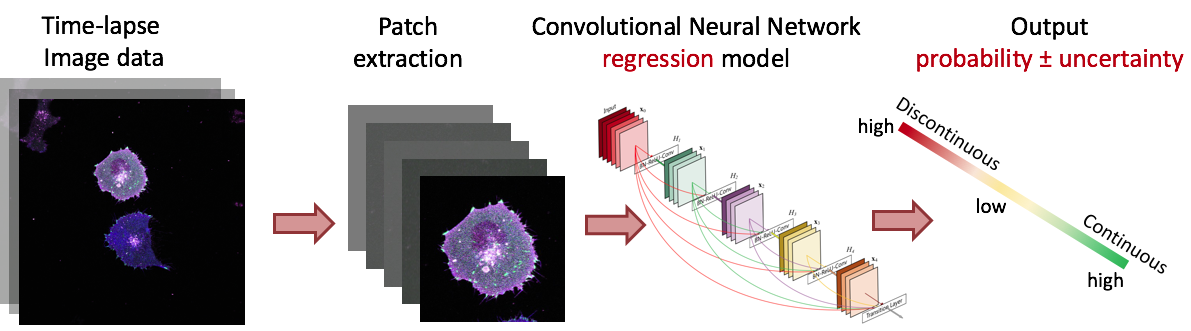
\includegraphics[width=1\linewidth]{paperImages/r4.png}}
        %  \vspace{2.0cm}
       % \centerline{(a) Result 1}\medskip
    \end{minipage}
    \caption[fig1]{The distribution of the predictions obtained by a classifier.} 
\end{figure}


\textit{\textbf{preprocessing}}: 
Due to high variability in the cell sizes, the images were first downsampled to 
a constant and equal size (512$\times$512$\times$3\,px) using Lanczos-3 kernel 
interpolation. 
For each annotated cell in each frame, we extracted 227$\times$2227$\times$3\,px 
patch from the centroid to include sufficient contextual information as an input 
for the network model.
The input images are then preprocessed by normalizing to zero mean and unit 
standard deviation. 

% \subsection{Label annotations}
% \label{subsec:annotation}
\textit{\textbf{Weak supervision label assignment}}: 
Our annotations are noisy as manually characterizing the behavior of mesenchymal cell migration 
modes with a high confidence is challenging because of their inherent switching properties. 
Given the noisy behavior of the cells label, it is reasonable to describe the confidence regarding
predictions instead of directly predicting their migration modalities.
Motivated from\,\cite{ding2018weakly}, we thus introduce a weekly supervised learning based crtieria.
Unlike the former approach, we focus on transforming the classification problem into a regression 
problem by genrating probablistic labels from the descrete frame-wise labels.

As we are provided with discrete frame-wise labels, i.e., 
\{\textit{continous}\,and\,\textit{discontinous}\} for each single cell time-lapse sequence
in the training phase, the goal is to predict probabilitistic confindence for the training 
data, as well as for unseen testing data. To achieve that we linearly interpolate the frame-wise
labels of each cell.
Given a cell of length \textit{n} and its labels of length \textit{n'}, we linearly interpolate the 
labels in the continous range of 0 to 1 to assigning them to their corresponding 
\textit{n'/n} frames. 
The range 0\,-\,0.4 corresponds to \textit{continous} mode whereas the range 0.6-1 corresponds to
\textit{discontinous} mode; and both are linearly mapped for \textit{n'/n} frames.
The range between 0.41-0.59 corresponds to the region with less confident predictions, and also
characterizing the conditions when cell starts switching migration modalities.


% \subsection{Bayesian Uncertainity}
% \label{subsec:bayesian uncertainity}
\textit{\textbf{Bayesian Uncertainity}}: 
Uncertainties in Bayesian modeling are characterized as either aleatoric uncertainty 
capturing noise inherent in the observations or epistemic uncertainty accounting for 
model uncertainty\,\cite{gal2016dropout}. %kwon2020uncertainty, 
%Estimating the uncertainty about a deep learning based prediction on a single sample 
%requires a distribution over possible outcomes. 
Model uncertainty for a given image can be obtained by keeping the dropout mechanism 
switched on at test time and performing multiple predictions, which is an approximation 
to the posterior distribution based on Bernoulli approximated variational inference
\cite{leibig2017leveraging, gal2016dropout}. 

We independently drop (with probability $p_{drop}$) the weights in all layers by drawing Monte Carlo 
(MC) sample from a Bernoulli distribution for each training sample \textit{x}.
%MC sampling is equivalent to performing dropout during training.
%, hence we get the Bayesian perspective as well for already trained models.
The predictive uncertainity is estimated by:

\begin{equation}
    \displaystyle
    \underbrace{\frac{1}{T} \sum_{t=1}^T diag(\hat{y}_t)-\hat{y}_t^{\otimes^2}}_{\textit{aleatoric}} +
    \underbrace{\frac{1}{T} \sum_{t=1}^T (\hat{y}_t-\bar{y})^{\otimes^2}}_{\textit{epistemic}}\;,
\end{equation}

where $\bar{y}=\sum_{t=1}^T{\hat{y}_t}/{T}$, $\hat{y}_t=Sigmoid\{f^{\theta_{t}}(x)\}$ and
\textit{T} refers to as the sampling rate.
We fixed \textit{T}= 50, as it was found in our case to be substantial for predictive mean 
estimation. 
The computation of MC samples for variational inference is fast and can also be applied to 
already trained networks.

\subsection{Networks}
\label{subsec:app 1.1}
We modified three existing networks, i.e., VGG16, Resnet 50, DenseNet, to
our need for comparison purposes.
We transformed each network model to be as a variational dropout network 
\cite{kingma2015variational}, i.e., each weight of a model has a dropout rate,
for Bayesian approximation. 
This allows us to perform approximate but efficient Bayesian inference by 
straightforwardly using existing network models.
Each convolutional layer was employed with ${\mathcal{L}_{2}}$ regularization 
to prevent overfitting, which is equivalent to putting a Gaussian prior 
on the network parameters, resulting in a maximum-a-posteriori (MAP) 
solution\,\cite{leibig2017leveraging}.

We employed the batch normalization operation specifically in the VGG16 
network model. 
We replaced the fully-connected layers with global average polling operation,
enabling us to use them with adaptive sizes of input. 
To obtain the regression output, we replaced softmax with sigmoid in the final
activation layer. 
The dropout rate ($p_{drop}$) for the initial layer was fixed to 0.1, which grow
exponentially at a rate of 0.05 for each subsequent layer. 
We found it to be a good compromise between getting a reasonable performance
and uncertainty measures.
% \subsection{Network Training}
% \label{subsec:training}
%  %For this reason, 

We trained the models in a 5-fold grouped stratified cross-validation scheme,
ensuring that the images from the same cell are not represented in both training
and testing sets. 
The number of images is larger for one migration mode than others, presenting
a class imbalance during training. 
The stratified sampling also ensures that the relative class frequencies are 
approximately preserved in each fold to deal with class imbalance issues.

The training was performed for 29,\,000 iterations with an initial learning rate of 0.01.
The weights were initialized using Glorot normal distribution \cite{glorot2010understanding} 
and the biases were set to zeros.
The weights were updated in a mini-batch of 4 samples using the ADAM optimizer.
The network was optimized by minimizing the logarithmic hyperbolic cosine error as loss function
and is defined as:
%rate of $1\mathrm{e}{-4}$ 
\begin{equation}
    {\mathcal{L}}(y,{\hat{y}})=\frac{1}{n}\sum_{i=1}^{n}\log(\cosh(y_{i}-{\hat{y}_{i}}))
\end{equation}
The network was implemented using Tensorflow backend in Keras, where the overall training took 
fifteen hours on a Titan X GPU.

% , where \textit{continous} mode span through 0-0.4 and \textit{continous} mode span through 0.6-1.
% ce region 
% We of both labels in a range 

% \{\textit{continous}


% A1;A2; :::;A$_{n}$'\} 
% for assigning them to their corresponding n/n' frames.
% The current cell labels are then transformed into a sequence with mixed probabilities generated 
% from linear interpolation.

% confidence the actual frame-wise

% per frame probablistic label generation from the 
% provided descrete labels of a given time-lapse sequence, and thereby
% transforming the classification problem into a regression problem. 

% predict the confidence regarding 
% the type of migration than discrete labels. 
% Therefore, we introduces a weekly supervised learning based crtieria, motivated from [Ref], 
% where we focus on probablistic predictions to describe the confidence regarding predictions.
% the discrete labels are transformed into probablistic labels to describe the 
% confidence regarding predictions.

% As the performance of deep learning models relies on the quality of the large hand-labeled 
% training data. These hand-labeled training sets are expensive and time-consuming to create — often 
% requiring person months or years to assemble, clean, and debug — especially when domain expertise is 
% required. Practitioners have increasingly been turning to weaker forms of supervision, such as 
% heuristically generating training data with external knowledge bases, patterns/rules, or other 
% classifiers. Essentially, these are all ways of programmatically generating training data—or, more 
% succinctly, programming training data. Many traditional lines of research in machine learning are 
% similarly motivated by the insatiable appetite of modern machine learning models for labeled training 
% data. 

% t is difficult to interpret cell behavior manually

% individual cells are known to not react uniformly
% to a treatment [12], thus generating subpopulations that may or may not be meaningful. 2) Some 
% treatments may have no effect at all, either because they are genuinely neutral treatments or
% because the treatment failed for technical reasons. In either case, forcing a CNN to find differences 
% where there are none may result in overfitting. 3) Sometimes different treatments yield the same cell 
% phenotypes, forcing a CNN to find differences between them may, again, result in overfitting to 
% undesired variation. 

% \subsection{Weak supervision label assignment}
% \label{subsec:weak-supervision}
% \textit{\textbf{Weak supervision label assignment}}: 
% The high quality deep learning models relies on the availability of on massive sets of hand-labeled 
% training data. These hand-labeled training sets are expensive and time-consuming to create — often 
% requiring person months or years to assemble, clean, and debug — especially when domain expertise is 
% required. Practitioners have increasingly been turning to weaker forms of supervision, such as 
% heuristically generating training data with external knowledge bases, patterns/rules, or other 
% classifiers. Essentially, these are all ways of programmatically generating training data—or, more 
% succinctly, programming training data. Many traditional lines of research in machine learning are 
% similarly motivated by the insatiable appetite of modern machine learning models for labeled training 
% data. 

% \textit{\textbf{Weak supervision explain}}:
% Clinicians often require a large time-lapse image sequence of cells to predict the cell migration 
% sub-modes with high confidence.
% Weak supervision is about leveraging higher-level and/or noisier input from subject matter 
% experts (SMEs). If we are approaching a challenging task that requires a complex model (i.e. one that 
% has a large number of parameters) then we generally need a training set too large to conveniently 
% label by hand. However, gathering enough training labels is a 
% major bottleneck in applying machine learning to new tasks. In response, there has been a shift towards 
% relying on weak supervision, or methods that can assign noisy training
% labels to unlabeled data. The key challenge in  automating weak supervision lies in 
% replacing the human reasoning that drives heuristic development. [tech-report-reef.pdf]

% we transformed the discrete labels into continous probablistic labels to perform regression.
% however, it is challenging for biologists to label a given cell with high confidence. Given 
% the noisy behavior of the labels, it is reasonable to predict the confidence regarding the type of 
% migration than discrete labels. Therefore, we introduces a weekly supervised learning based crtieria,
% motivated from [Ref]. Unlike the former approach, we focus on probablistic label generation from 
% given time-lapse sequence, eventually transforming the classification problem into a regression problem. 

% Given a time-lapse sequence of a single cell, in the training process, we are provided with discrete
% ground-truth labels for migration mode, i.e., \{cont and discont\}. The goal is to predict 
% probabilitistic output y in the training data with the given migration modes, as well as to predict 
% the actual frame-wise labels for unseen testing data.

% We start with a linear interpolation of per frame labels for each cell.
% Given a cell of length \textit{n} and its labels of length n', 
% we linearly interpolate the probabilities of both labels in a range \{A1;A2; :::;A$_{n}$'\} 
% for assigning them to their corresponding n/n' frames.
% The current cell labels are then transformed into a sequence with mixed probabilities generated 
% from linear interpolation.

% similar approach is explored in [Ref]. Unlike them, our approach focuses on probablistic label 
% generation from given time-lapse sequence to transform the classification problem into a plain regression
% problem. 

% we do not sample images,
% but instead sample class labels uniformly at random. From each sampled label we then select a random 
% image to create training batches, following the practice in [17].


% \subsection{Approch 1 from Static image data}
% \label{subsec:app 1}

% \subsection{Approch 2 from temporal image data }
% \label{subsec:app 2}

% \subsubsection{Approch 2.1 Networks}
% \label{subsubsec:app 2_1}
% VGG, Densenet, Resnet

% Estimating the uncertainty about a deep learning based prediction on a single sample 
% requires a distribution over possible outcomes. 
% Using dropout networks, where subsets of units are inactivated during 
% training to avoid overfitting, we compute an approximation to the posterior 
% distribution by sampling multiple predictions with dropout turned on. This allows us 
% to perform approximate but efficient Bayesian inference by using existing network models 
% in a straightforward way. Another advantage of this approach is that it can be applied to 
% already trained networks. [41598-2017-Article-17876.pdf]

% Bayesian convolutional neural networks with Bernoulli approximate variational inference. In practice, equation
% (2) is intractable and a common way to find approximating solutions is via variational inference.
% The integral in eq.(4) is still intractable and therefore approximated with Monte Carlo sampling. 
% This results in the conventional softmax loss for dropout networks, for which units are dropped by drawing 
% from a Bernoulli prior with probability $p_{drop}$ for setting a unit to zero. The KL term in (4) was 
% shown to correspond to a L2-regularization term in dropout networks.
% We use xx as a shorthand notation for stating that in order to decide whether a unit is dropped, we independently
% sample from a Bernoulli distribution (with probability $p_{drop}$) for each unit in all layers for each training sample.
% Note that Monte Carlo sampling from q(.) is equivalent to performing dropout during training, hence we get the
% Bayesian network perspective as well for already trained models.
% Obtaining model uncertainty for a given image is as simple as keeping the dropout mechanism switched 
% on at test time and performing multiple predictions. The width of the distribution of predictions is 
% then a reasonable proxy for the model uncertainty. 

% Obtaining model uncertainty for a given image is as simple as keeping the dropout mechanism switched on at test 
% time and performing multiple predictions. The width of the distribution of predictions is then a reasonable proxy 
% for the model uncertainty
% In short: the wider the distribution, the less the different subnetworks agree. Regarding the choice of T, we fixed 
% it to T= 100 because it was shown by to suffice for reducing the test error by improving the quality of the predictive 
% mean estimation. Different values for T affect how well the true population moments $\mu_{pred}$ and $\sigma_{pred}$
% can be estimated: Var($\hat{\mu}_{pred})=\frac{\sigma{^2}_{pred}}{T}$.
% It should however be noted, that the computation of MC samples is extremely fast: The test predictions could 
% be performed in parallel, but even a serial implementation takes less than 200ms per image. Hence there is no 
% practical reason to compute fewer testing samples than the T= 100 used to obtain the results presented here.

% the low voltage (25keV) tabletop 
% MiniTEM\footnote{Vironova AB, Stockholm}. Low- and high-resolution (LR and HR) images of the same areas 
% of a calibration grid with line grating replicas with latex spheres, and the images had a FoV of 6 and 
% 1.5\,$\mu$m, respectively. To establish corresponding HR\,-\,LR dictionary pairs for training and 
% evaluation, a number of preprocessing and registration steps were performed. As preprocessing, background 
% subtraction was applied within the MiniTEM SW using an aggregated background image, and the images were 
% then linearly resampled to 8-bits after cropping the 0.01$\%$ of the brightest pixels to exclude hot pixels.
% Rigid HR/LR registration (HR downsampled to LR) was done using the Harris point detector, the log-polar 
% magnitude point descriptor and RANSAC as describe in detail in \cite{matuszewski2017logPolarD}. Elastic 
% registration after upsampling the matching region in the LR image was then performed using bUnwarpJ 
% \cite{arganda2008bUnwarpj} in ImageJ, using the default settings and the HR as the moving image (i.e., 
% the one that is deformed). In total, 871 dictionary image pairs were created for the calibration grid, 
% which were then cut into non-overlapping 256$\times$256 px patches. To investigate the effect on performance 
% when training using real versus synthetic data, a synthetic dataset was created by downsampling the HR images 
% using nearest neighbor to generate corresponding LR images. 

% \subsection{Image acquisition}
% \label{subsec:acquisition}

% The High resolution images of H1299 (human non-small lung carcinoma) cell is acquired with 
% Nikon A1R confocal microscope using a PlanApo VC 60X/1.4 NA oil-immersion objective (Nikon, 
% Amsterdam, Netherlands). Images are acquired for 8–10 hr at 5 min intervals with a pixel 
% resolution of 0.21 m. 
%FEEL FREE TO EDIT===
% The proposed network learns an end-to-end mapping between the LR-HR image pairs by encoding local and global 
% representations. It jointly exploits the feature sharing capabilities of both dense \cite{huang2017DenseCNN} 
% and residual connections \cite{he2016identity} to enhance the structural information in the reconstructed 
% output. The dense skip connections contrast the residual skip connections regarding feature reusability. 
% Residual connections directly add the encoded representations instead of concatenation as in DenseNet 
% \cite{huang2017DenseCNN}. Compared to the original DenseNet, we removed all the pooling and batch normalization 
% layers, and used fewer dense modules which greatly reduces the total number of trainable parameters. 

% % Mearging
% Further, we upscaled the encoded representations using sub-pixel convolutions \cite{shi2016real} to overcome 
% the problem with checkerboard artifacts and to achieve 4$\times$ SR reconstruction. Contrarily to this, most 
% of the previous CNN-based methods upscale the low-level descriptions by employing transposed convolution 
% (or deconvolution) operations \cite{dumoulin2016guide}. However, multiple transposed convolution layers 
% can easily lead to uneven overlap (or checkerboard artifacts) on a variety of scales, which limits the 
% network's representational capacities. 

% %\subsection{Network structure}
% \textbf{\textit{Network structure:}} Our network combines three different types of modules: a generic 
% feature encoder module, densely-connected residual mapping modules, and an upscaling module. 
% % Combining the first module, since it is very small
% The feature encoder module encodes low-level representations by applying two convolution operations on the 
% input LR images of 64$\times$64 px. Both convolution layers generate 32 feature maps using 3$\times$3 kernels
% and are followed by rectified linear units (ReLU) activations. The input is padded with zeros to keep the 
% image size fixed throughout the module. 

% A densely-connected residual module encodes multiple levels of representations for improved edge 
% reconstruction. The proposed network employs eight such modules (decided through empirical testing). 
% Each module consists of five locally dense-connected convolution layers  to generate 32 feature maps 
% using 3$\times$3 kernels except the last layer which uses 1$\times$1 kernel. Every layer is followed 
% by ReLU activations. The local dense connections simultaneously encode both the low- and the high- level 
% structural representations by concatenating the output of a forgoing convolution layer to the input of 
% all the subsequent layers. The concatenated feature maps are then convolved with the 1$\times$1 kernel 
% to reduce the computational complexity of the network. The residual mapping (i.e., addition) is then 
% performed by summing the resultant feature maps of the current module with its input to enhance the 
% structural representations of edges.

% The upscaling module employs a sub-pixel convolution operation to upscale the concatenated 
% representations obtain from the eight densely-connected residual modules. The concatenated output is then 
% convolved using 1$\times$1 and 3$\times$3 kernels to generate ReLU activated 32 feature maps. The 1$\times$1 
% convolutional kernel combines the different levels of abstracted representations. To enforce the network 
% to encode rich descriptions, a global residual mapping \cite{ledig2017photo} is performed by adding the 
% resultant feature maps with the output of the feature encoder module. Once the local and global 
% representations are encoded, the sub-pixel convolution operation and ReLU activation are applied to 
% generate 32 upscaled feature maps using 3$\times$3 kernels. The final convolution layer is then applied 
% using 3$\times$3 kernels to generate the reconstructed SR output of 256$\times$256 px.

%\subsection{Network training}
%\textbf{\textit{Network training:}} 

%===========================================================================
%===========================================================================
\section{Experiments and results}
\label{sec:exprm}

% Cell protrusion is morphodynamically heterogeneous at the subcellular level. However, the mechanism of cell 
% protrusion has been understood based on the ensemble average of actin regulator dynamics. Elucidating the
% Cell protrusion is driven by spatiotemporally fluctuating actin assembly processes, and is morphodynamically 
% heterogeneous at the subcellular level1–3. Elucidating the underlying molecular dynamics associated with 
% subcellular protrusion heterogeneity  is crucial to understanding the biology of cellular movement since 
% protrusion determines the directionality and persistence of cell movements or facilitates the exploration of 
% the surrounding environment. Advances in computational image analysis on live cell movies have allowed us to 
% study the dynamic aspects of molecular and cellular events at the subcellular level. However, the significant 
% degree of heterogeneity in molecular and subcellular dynamics complicates the extraction of useful information 
% from complex cellular behavior. Although some studies have examined the cellular heterogeneity of the migratory 
% mode, subcellular protrusion heterogeneity has not yet been addressed. CNN can potentially identify distinct 
% subcellular protrusion phenotypes based on a spatiotemopral analysis of heterogeneous subcellular
% protrusion velocities extracted from live cell movies (Figs. 1a–c). It can associate each protrusion phenotype with 
% pertinent actin regulator dynamics by comparing the average temporal patterns of protrusion velocities with those of 
% actin regulators[s41467-018-04030-0.pdf]

% We explored two variants of our proposed network, differing only that one was trained on synthetic and 
% the other on real LR-HR image pairs. The two variants are referred to as S$_8$ and R$_8$ corresponding to 
% the synthetic and real data, respectively. The subscript \textit{eight} indicates the number of densely 
% connected modules used in the network. We analyzed the performance gain by varying the number of these 
% modules in a range of 8\,-\,24  with an interval of 4. Here, peak-signal-to-noise ration (PSNR) in 
% decibel (dB) and structural similarity index (SSIM) are used as the performance measures. The observed gain
% for higher depths was minimal ($\Delta$PSNR\,$<$\,1dB, and $\Delta$SSIM\,$<$\,0.005). Thus, we opted and 
% evaluated the performances using \emph{eight} modules. The quantitative results on the independent test 
% dataset, consisting of 41,\,503 sample images, for the S$_8$ and R$_8$ variants of our proposed network 
% compared to classical interpolation techniques are presented in Table \ref{tab:resultCalibgrid}, examples 
% for qualitative visual comparison are shown in Fig.\,\ref{fig:resultCaligrid}. 

% %======================================
% % Result table on test dataset for calibration-grid 
% %======================================
% %\input{tables/tabTestResultCalibrationGrip.tex}
% %====================================

% The results show that the network variants, as expected, are superior to the classical interpolation 
% techniques. The network trained on real data perform better than the one trained on synthetic data. 
% The lower performance of S$_8$ compared to R$_8$ illustrates the benefit and importance of training 
% on real data to capture the system's imaging model and characteristics. On the other hand, the lower 
% performance of S$_8$ can also be explained as variation differences in the testing and training datasets, 
% since the trained model can handle contrast and noise variability, which is not present in the testing data. 
% However, the qualitative results eliminate this argument (see, Fig.\,\ref{fig:resCalibgrid_VAS8} and 
% \ref{fig:resCalibgrid_VAR8}) which clearly shows the advantage and benefit of using real data when deploying 
% deep learning techniques in real imaging systems.

% Result figure on test dataset for calibration-grid 
%======================================
%\input{figures/resultImgsCalibrationgrid.tex}
%======================================

%======================================
%\input{paperImages/r1.png}
% \begin{figure*}[ht]
% 	\centering
% 	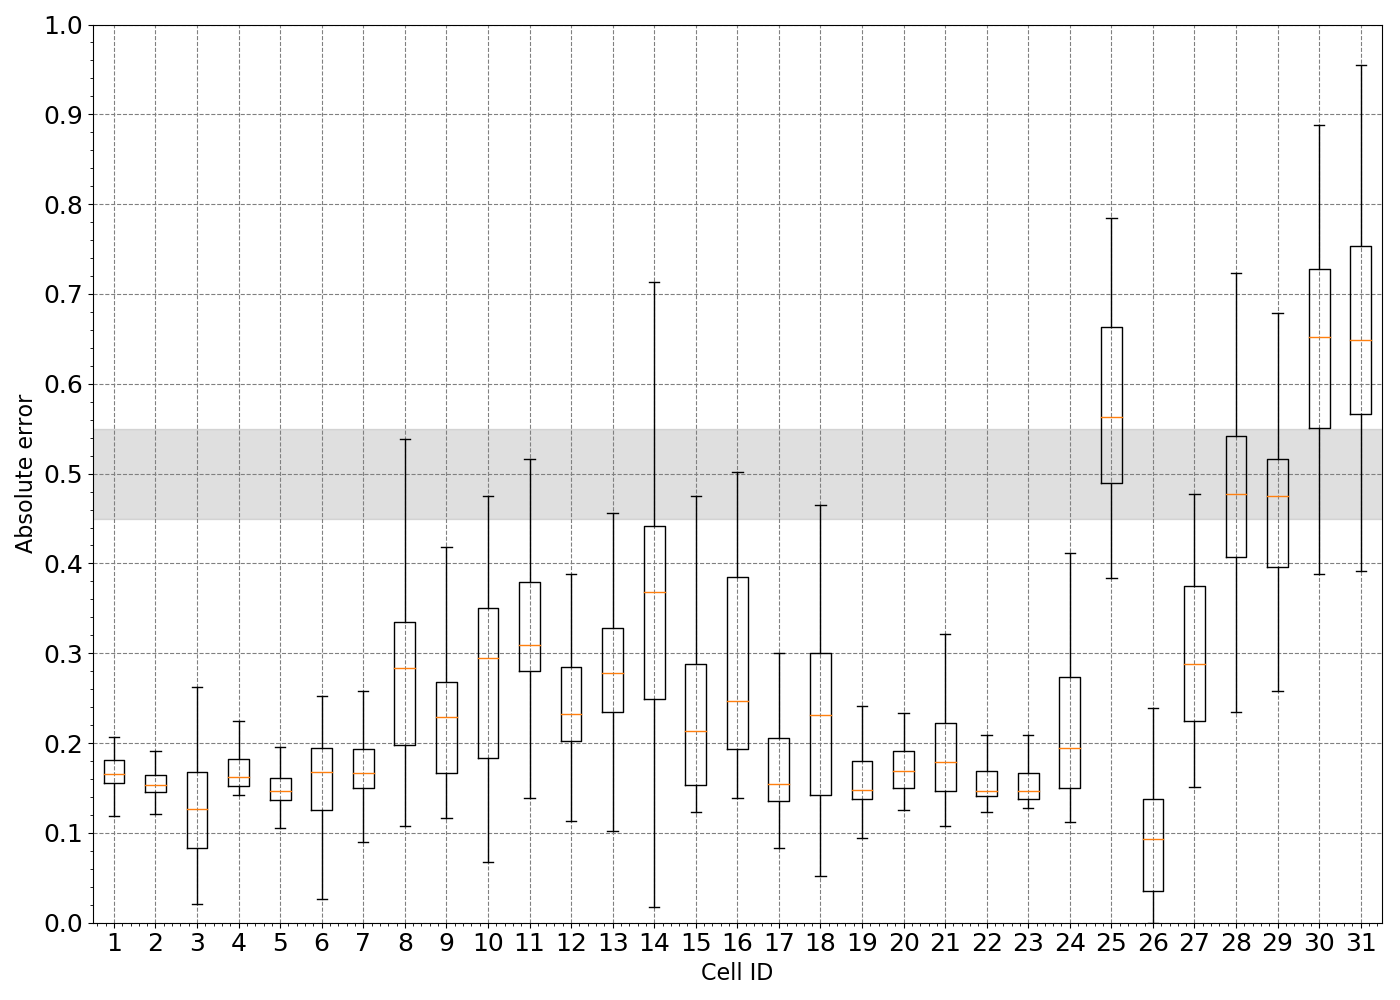
\includegraphics[width=0.5\linewidth]{paperImages/r3.png}
%     \caption[fig3]{The distribution of the predictions obtained by a classifier.} 
% 	\label{thres_im}
% \end{figure*}

% \begin{figure*}[ht]
% 	\centering
% 	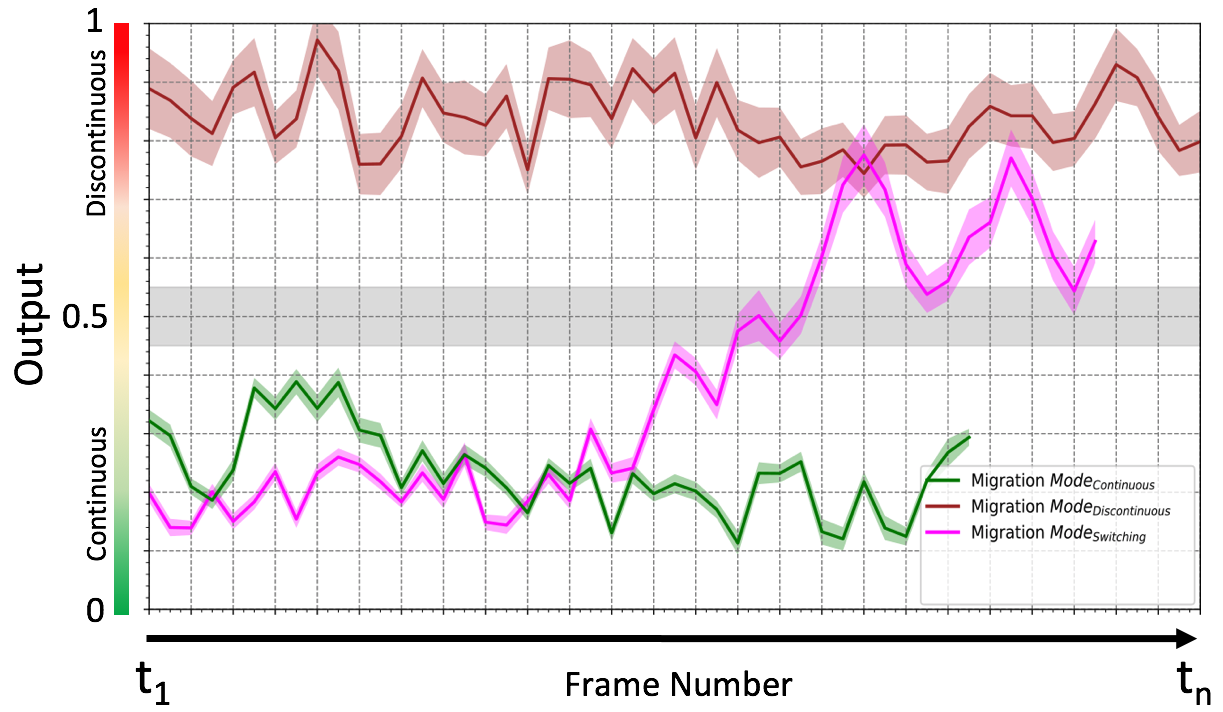
\includegraphics[width=0.8\linewidth]{paperImages/r1.png}
%     \caption[fig1]{The distribution of the predictions obtained by a classifier.} 
% 	\label{thres_im}
% \end{figure*}


\begin{figure}[b]
\begin{minipage}[b]{1.0\linewidth}
    \centering
    \centerline{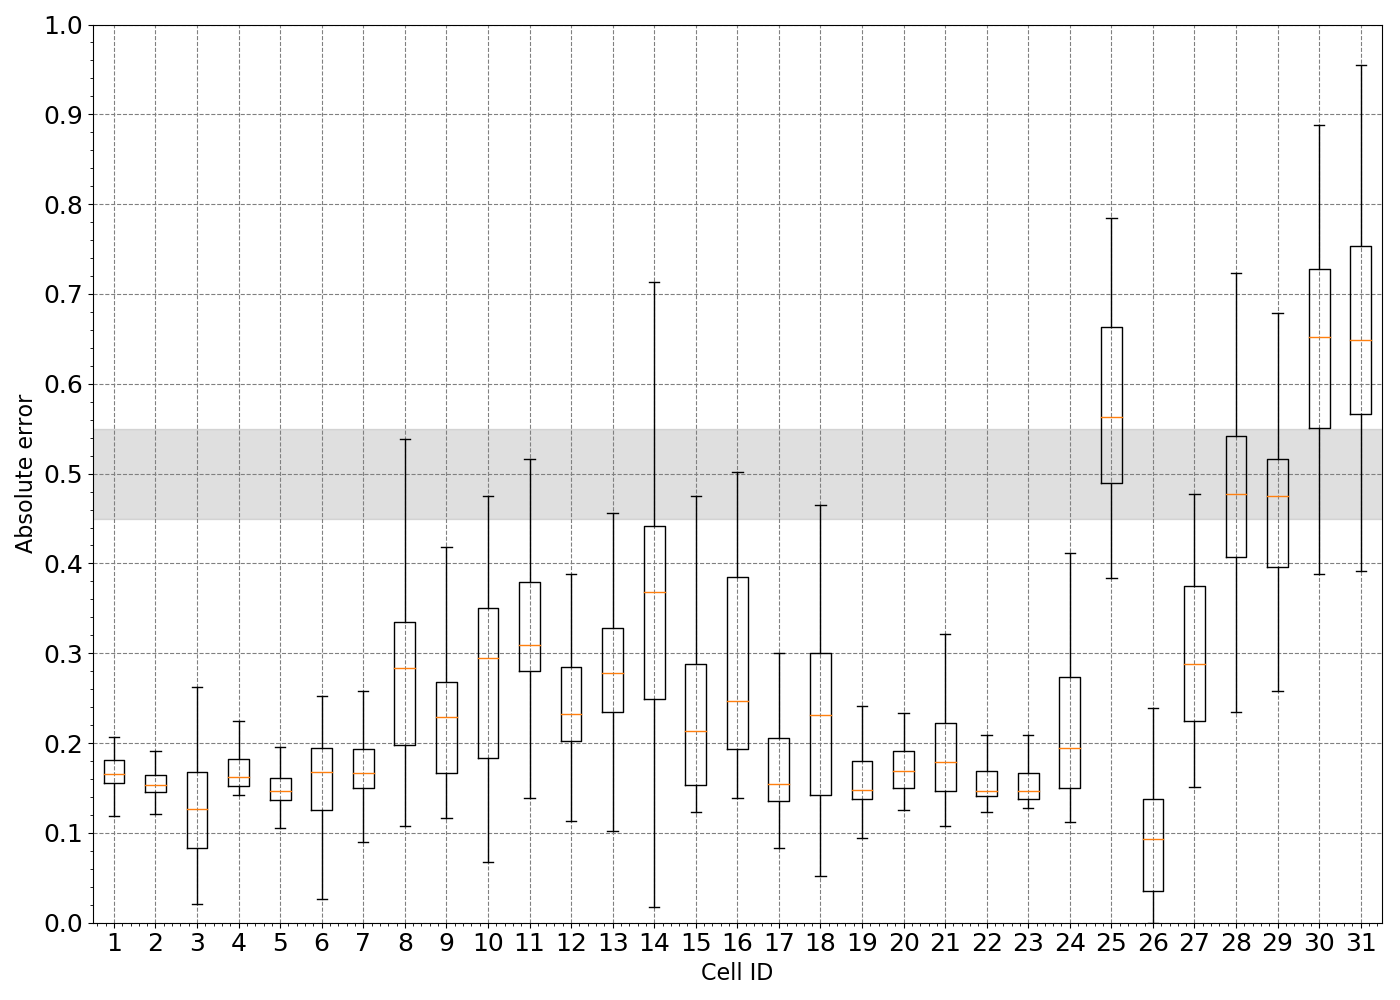
\includegraphics[width=1\linewidth]{paperImages/r3.png}}
    %  \vspace{2.0cm}
   % \centerline{(a) Result 1}\medskip
\end{minipage}
\caption[fig2]{The distribution of the predictions obtained by a classifier.} 
\end{figure}

\begin{figure}
    %\begin{subfigure}{.5\textwidth}
      \centering
      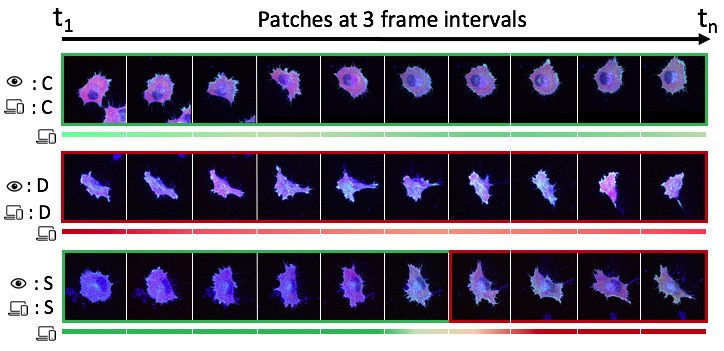
\includegraphics[width=1\linewidth]{paperImages/r2.png}
      \caption{1a}
      \label{fig:sfig1}
    %\end{subfigure}%
\end{figure}    
\begin{figure}
    %\begin{subfigure}{.5\textwidth}
      \centering
      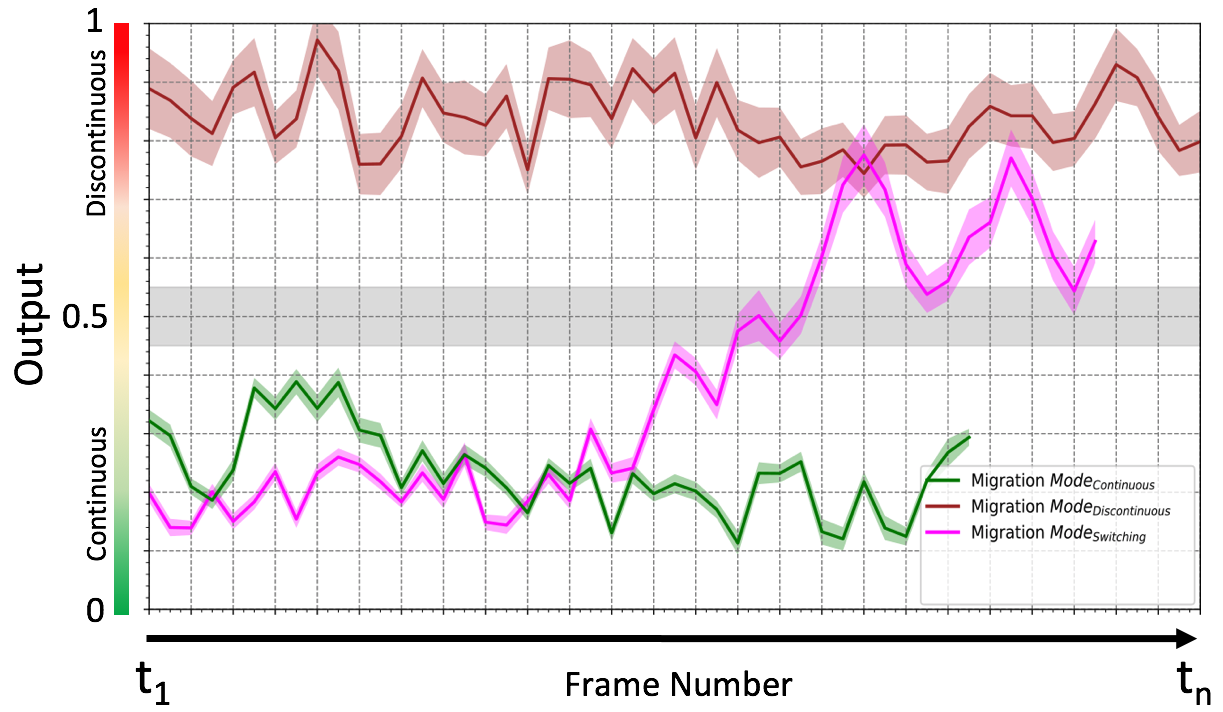
\includegraphics[width=1\linewidth]{paperImages/r1.png}
      \caption{1a}
      \label{fig:sfig1}
    %\end{subfigure}%
\end{figure}    
    % \begin{subfigure}{.5\textwidth}
    %   \centering
    %   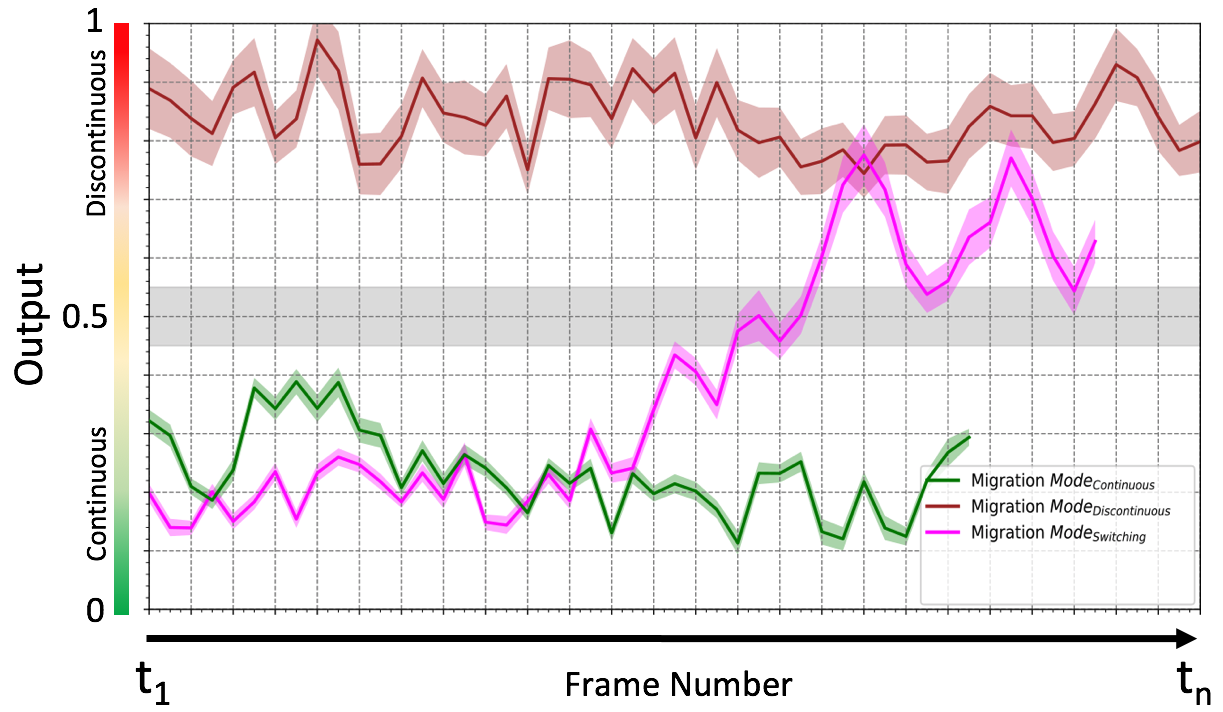
\includegraphics[width=\textwidth]{paperImages/r1.png}
    %   \caption{1b}
    %   \label{fig:sfig2}
    % \end{subfigure}
    % \caption{plots of....}
    % \label{fig:fig}
    % \end{figure}

% \begin{figure*}[ht]
% 	\centering
% 	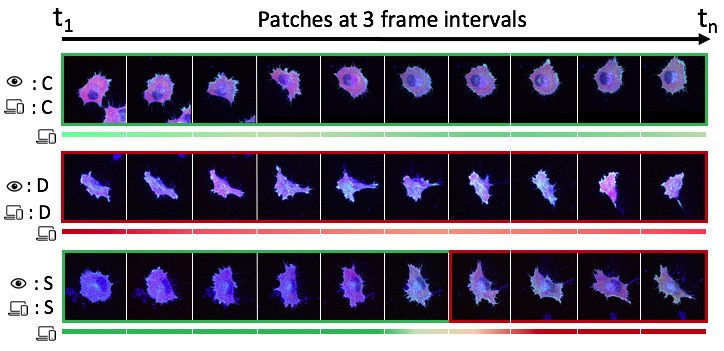
\includegraphics[width=0.8\linewidth]{paperImages/r2.png}
%     \caption[fig3]{The distribution of the predictions obtained by a classifier.} 
% 	\label{thres_im}
% \end{figure*}
% \begin{figure*}[ht]
% 	\centering
% 	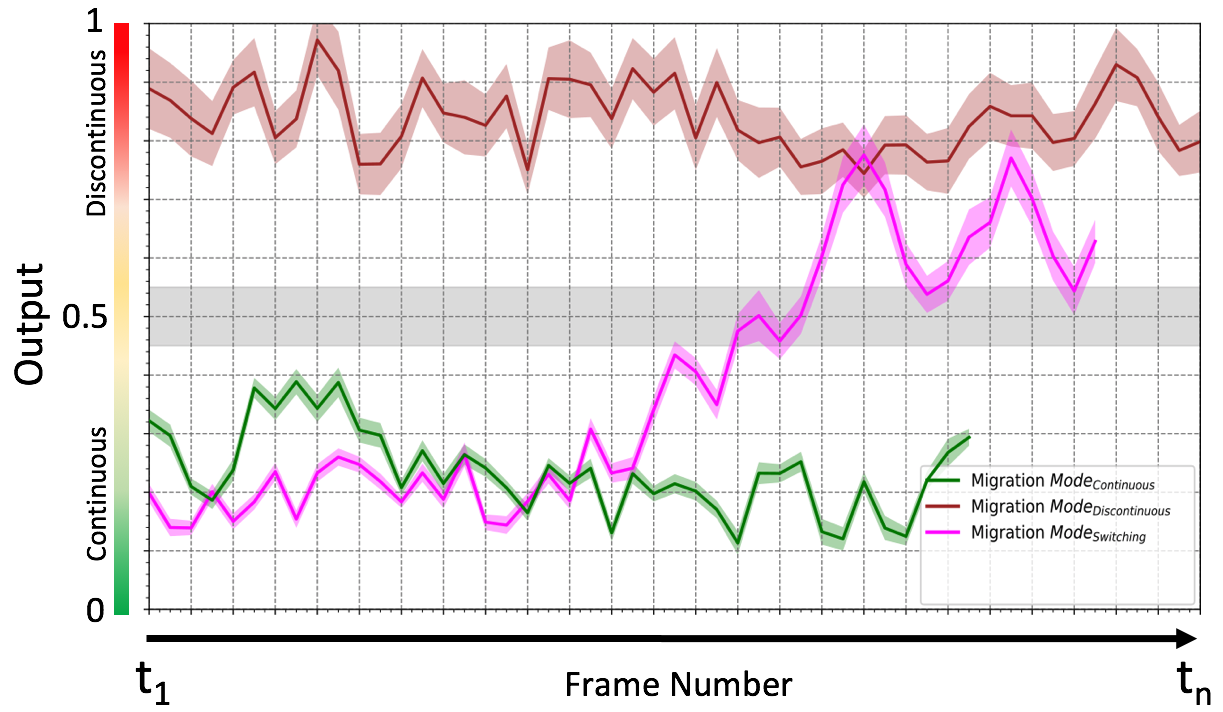
\includegraphics[width=0.8\linewidth]{paperImages/r1.png}
%     \caption[fig4]{The distribution of the predictions obtained by a classifier.} 
% 	\label{thres_im}
% \end{figure*}
    %
    % \begin{minipage}[b]{.48\linewidth}
    %   \centering
    %   \centerline{\includegraphics[width=4.0cm]{image2}}
    % %  \vspace{1.5cm}
    %   \centerline{(b) Results 3}\medskip
    % \end{minipage}
    % \hfill
    % \begin{minipage}[b]{0.48\linewidth}
    %   \centering
    %   \centerline{\includegraphics[width=4.0cm]{image3}}
    % %  \vspace{1.5cm}
    %   \centerline{(c) Result 4}\medskip
    % \end{minipage}
    % %
    % \caption{Example of placing a figure with experimental results.}
    % \label{fig:res}
    % %
%
%======================================
% To investigate the domain adaptive capacity of our proposed network, we applied the S$_8$ and R$_8$ variants 
% on downsampled cilia images (see image data section) and visually compared the result with high-resolution 
% images of the same objects. Since the cilia images have an inverted intensity profile relative to the 
% calibration grid images (i.e., cilia are the dark objects on a bright background, whereas the calibration 
% grid has bright details on a darker background), we also fed the inverted cilia images into the network. 
% In the first look, the results from the model trained on synthetic data gives an impression of achieving 
% better quality (see, Fig.\,\ref{fig:resCiliagrid_VAS8psd}). However, there are "ghost effects" and impacts 
% from the training data can be seen in the reconstructed cilia images. For the inverted input, the network 
% trained with real data results into a descent quality image while reconstructing the most subtle details 
% (see inset: Fig.\,\ref{fig:resCiliagrid_HRpsd} and \ref{fig:resCiliagrid_ngVAR8psd}, the double border 
% effect). The other variations of network and inputs clearly failed to recover such details. We observed 
% that the reconstruction performs better for inverted cilia images since the bright worm-like features 
% of training data matches to the structural appearances of cilia. %and thereby potentially resulting in better reconstruction.
%The reconstruction works better for the inverted cilia images and bright worm-like features in the images looking like the details in the training data are enhanced. 
% Result figure on partially synthetic cilia dataset (04-01)

%===========================================================================
%===========================================================================
\section{Discussion and Conclusion}
\label{sec:concl}

The proposed model yields a substantial performance on the image dataset with different fibronectin 
concentration levels and thereby showing a great potential to be used as an automated method for 
large-scale live cells screening. However, whether the inclusion of temporal information improves the 
prediction performance or not is remained to be shown. Next, to reveal how and why CNN models can predict 
the migration modes, we will visualize the features of the cell images that were learned by the CNN 
models and contributed to their prediction: e.g., the protrusions and trailing edge. The proposed model 
yields the probability with an uncertainty that describes the confidence regarding predictions. 
If we manage to predict  the migration behavior with just single frame then the phototoxity and staining 
can be overcome which is good in general.

% Overall, the soft boundary mechanism stands for the idea of using a mixture of probabilities to 
% represent the boundary between two different actions. We believe such representation and mechanism 
% are important in the field of action modeling, where you can not always tell the exact changing 
% point of an action, and thus worths further exploration. It features an iterative training procedure 
% with transcript refinement and soft boundary assignment. We note that, although our change is simple, 
% it is effective. During experiments, we found such setting usually gives a bonus on performance than 
% simply up-sample transcript to video length by hard assignment.

Here, we demonstrate that a CNN can prospectively predict the migration sub-mode from a single 
image observation of a cell, and thereby overcoming the challenges of high photo-toxicity while 
minimizing the data acquisition efforts and data storage requirements. Furthermore, it addresses the 
inter- and intra-observer prediction variability by providing the model uncertainties while yielding 
high accuracy. For comprehensive and adequate quantitative analysis, this work focuses on harnessing 
the discriminative capabilities of deep learning based methods to perform real-time classification of 
two migration modes, and thereafter, to increase the understanding of underlying phenomenon that 
influences the cellular organization of each migration mode. Automation can help to reduce the noise 
induce by the multiple manual intervention. 
The study results showed the CNNs with automatically generated features can achieve desirable performance 
in cell migration mode prediction with just using a single cell observation.

This paper proposes an automatized approach for mesenchymal 
cell migration mode prediction. It discriminates candidates by encoding the morphological representations 
from the single cell observations (image patches), and also by encoding the spatiotemporal 
representation from image sequences.  CNN and its variants offer 
several advantages in predicting cell migration modalities. The migration processes usually span 
several consecutive images, the migration modes can be predicted after considering both spatial and 
temporal information from adjacent image frames. 

Given the spatiotemporal behvaior of imaging data, one preferred choice would have been exploiting recurrent 
neural networks (RNNs) to learn morphological and temporal representations. 
However, optimzing RNNs is complex due to the gradient vanishing and exploding problems, and computationally expensive 
and time-consuming training process over large time-lapse image sequences. 
Also, it is not trivial optimizing the additional hyperparameter, i.e., the ammount of temporal context needed
for substantial perfromance gain. 

% In this work, we present a proof of concept for broader adoption of CNN-based methods in real-time 
% imaging setting. The experimental results show that the model trained using real data produces better results 
% than synthetic for the calibration grid. Nevertheless, this is expected since the network learns the imaging 
% system modelling and realistic noise conditions better to derive the mapping function from LR to HR 
% reconstruction. While testing for the domain adaptation capability, we noticed the appearance of 
% ghost artifacts, i.e., worm-like structures similar to the pattern on the calibration grid which was 
% not present in the data initially. We believe, fine-tuning the derived model (transfer learning) or 
% including a smaller subset of different types of samples in the training data will likely improve the 
% results. Further, covering a broad spectrum of simple variations comprising of potential disparities of 
% the real settings during the data augmentation can substantially boost the performance, as demonstrated 
% with the inverted image experiment. From the results for synthetic and real data on cilia indicate that 
% including both synthetic and real data in training dataset could improve the performance most since the 
% synthetic data is downsampled and has an exact match (representing a perfect system) with the HR. 

% In conclusion, we have shown the benefit and importance of using the real data and our experiments 
% establish the possibility of using a generic network for reconstructing super-resolution TEM images 
% when trained for specific applications. Using such super-resolution reconstruction will allow for 
% achieving high-resolution image data in shorter time along with less data handling and storage 
% requirements overheads, and hence make TEM image acquisition and corresponding data handling more efficient.

%===========================================================================
%===========================================================================
  
% In this study, we investigate whether CNNs can potentially encode discriminative morphological/spaital
% representations
% from a static cell observation to predict different migration modes in confocal microscopy image data. 
% how much temproal context is needed for substantial perfromance gain
% optimizing the length of timesteps to capture the temporal context amount of tempral context needed to determine the optimal
% substantial performance to capture the temporal context.
%Also, it is often not trivial to determine the optimal temproal context needed for perfromance gain.
%and not straightforward due to multiple reasons.
%Hence, we strive for simplicity by learning  morphological representation 
% using static observations of cells.
% It is often the case that the given ground-truth labels are noisier. \textbf{[fd254b271.pdf]} Such situation, for instance, 
% occurs when the human annotators are unable to annotate the migation mode with high confidence.

% With a hypothesis that can CNNs encode the morphological/spaital representations from a static cell observation, 
% we thus strive for simplicity by learning discriminative morphological representation 
% for probablistic prediction of different migration modes using static observations of cells.

 
% However, we hypothesize that it is still possible to 
% deduce the migration mode just from a static cell observation. The proposed model can automatically 
% learn robust and representative features, including the static, spatial, and temporal ones, directly 
% from captured data. [1-s2.0-S0950705117303738-main.pdf]

% \textit{\textbf{6. talk about single frame prediction motivaition and benefits}}\\
% \textit{\textbf{7. talk about why LSTM are not used and whats wrong with recurrent}}\\
% \textit{\textbf{8. talk about contribution}}\\
% \textit{\textbf{Possible Solution}}: 

%\textit{\textbf{Weak supervision}}: 
%\subsection{Problem}
%\label{subsec:prob}
%\subsection{Possible Solution}
%\label{subsec:sol}
%\textit{\textbf{4. talk about annotation challenges weak labels}}\\
%\textit{\textbf{5. talk about baysian uncertainity}}\\

% In biomedical imaging applications, assessment of uncertainty could potentially reduce untoward outcomes 
% due to suboptimal decisions. 

% , and 
% thus weak supervison are a good fit to such situations.
% W

% Lately, convolutional neural networks (CNNs) based solutions have reasonably shown a high sensitvity 
% on complex biomedical data analysis problems \textbf{[Gupta et al. 2019]}. 

% Weak supervision is about leveraging higher-level and/or noisier input from subject matter 
% experts (SMEs). If we are approaching a challenging task that requires a complex model (i.e. one that 
% has a large number of parameters) then we generally need a training set too large to conveniently 
% label by hand. With an increasing amount of biomedical image data, it is challenging to perform 
% human-level annotation accurately, and thus are a good fit for weak supervision to derive interpretable 
% quantification. If we have domain expertise to leverage, then weak supervision provides a simple, 
% model-agnostic way to integrate it into our model. However, gathering enough training labels is a 
% major bottleneck in applying machine learning to new tasks. In response, there has been a shift towards 
% relying on weak supervision, or methods that can assign noisy training
% labels to unlabeled data. The key challenge in  automating weak supervision lies in 
% replacing the human reasoning that drives heuristic development. [tech-report-reef.pdf]
% A key bottleneck in building a 
% model is that they typically require carefully curated annotated training data. Acquiring such data 
% is an expensive, time-consuming annotation effort. It is often the case that the given ground-truth 
% labels are noisier. Such situation occurs when the human annotators are unable to annotate a cell with
% high confidence. 
% Inaccurate supervision concerns about the situation where the supervision information
% is not always ground truth; in other words, some label information may suffer from errors. Supervised 
% learning techniques have achieved great success when there is strong supervision information like 
% large amount of training examples with ground-truth labels. In real tasks, however, collecting 
% supervision information requires costs, and thus, it is usually desired to be able to do weakly 
% supervised learning. [fd254b271bcc2fb7e2a62d75.pdf]

% The inception of CNNs has revolutionized the field of computer vision and image analysis. Deep learning 
% based automatized and integrated algorithmic solutions have been shown to achieve high performance on 
% complex scientific data analysis problems that previously required domain experts. Despite the 
% outstanding performances of CNNs for cytometric image analysis[Gupta et al. 2019], less attention has 
% been paid to probabilistic interpretations of the predictions via uncertainty quantification. 
% Absences of sufficient understanding of model outputs may provide suboptimal results. 

% In Bayesian modeling, uncertainties are characterized as either aleatoric 
% uncertainty capturing noise inherent in the observations or epistemic uncertainty which accounts for 
% model uncertainty.[eb54c133570186f377252b1ce610213ed8a7b241.pdf]


% Automated algorithms can rapidly quantify the biological and morphological differences at the 
% single-cell level. However, such qunatitative analysis strive for the integrated 
% algorithms with a high sensitivity. 

%Automatized computational methods and tools have therefore become essential 

% The availability of carefully annotated image databases and the topological advancements have realized 
% CNNs as the foremost technique of interest for many computer vision 
% and image analysis problems. Despite the substantiated progress in the designing of neural network 
% topologies, their implication in biomedical experiments are still confined due to lacking of the 
% large amount of carefully annotated data.
% A key bottleneck in building a deep learning model is that they typically require carefully curated 
% annotated training data. Acquiring such data in biomedical field is an expensive, time-consuming effort. 

% Despite the outstanding performances of CNNs for cytometric image analysis[Gupta et al. 2019], less attention has 
% been paid to probabilistic interpretations of the predictions via uncertainty quantification. Absences 
% of sufficient understanding of model outputs may provide suboptimal results. Estimating the uncertainty 
% about a machine learning based prediction on a single sample requires a distribution over possible 
% outcomes, for which a Bayesian perspective is principled. Bayesian approaches to uncertainty estimation 
% have indeed been proposed to assess the reliability of clinical predictions but have not been applied 
% to the large-scale real-world problems that DNNs can target.  Uncertainty quantification of predicitons 
% can lead to a more informed decision, and the quality of prediction can be improved. In biomedical 
% imaging applications, assessment of uncertainty could potentially reduce untoward outcomes due to 
% suboptimal decisions. 


% However, their 
% implication/realization is often confined due to two foremost reasons.
% 1) lacking of the large amount of carefully annotated data.
% It is often the case that the given ground-truth labels are noisier. Such situation occurs when the human 
% annotators are unable to annotate cells with a high confidence.
%which often confined by the two foremost challenges:. The high sensit 

% Leveraging the convolutional neural networks (CNNs) for encoding the discriminative representation 
% may improve the quality and sensitivity of the signal measured in biological experiments. 
%  Strategies such as transfer learning and data augmentation 
% can be considered as potential solutions to the lack of labels. 


%\textit{\textbf{Problem}}: 

% A complete understanding of complex mechanism underlying mesenchymal migration process across several spatial 
% and temporal scales is indeed crucial to derive an adequate quantification for single cell-based 
% analysis [\textbf{REF}].
% Thanks to \textit{Systems Microscopy} which holds a great potential to elucidate the spatiotemporal complexities 
% of cell migration modalities. It is a new and growing approach facilitating systems biology by 
% analyzing the quantitative recording of multiple dynamic cellular responses of living, individual 
% cells over time using computational algorithms. [\textbf{REF}]


% Automatized and integrated algorithms are thus highly desired to facilitate mesenchymal migration 
% sub-modalities prediction.
% The overabundance of experimental data makes a manual prediction of 
% migration modes challenging (time-consuming and tedious) and eventually often leads to erroneous 
% observations. Clinicians often require a large time-lapse image sequence of cells to predict the cell 
% migration sub-modes with high confidence.
% Manual classifications of migrating cells into the different 
% modalities have previously been performed by analysing long time-lapse movies from migrating cells. 
% These movies are often acquired during several hours, 8 hours or more, generating large amount of data
% (Shafqat-Abbasi et al. eLife 2015).  

% Deep convolutional neural networks (CNNs) can encode powerful visual representations when exposed 
% to a substantially larger labeled training dataset. 

% In microscopy images, modeling spatiotemporal features are important for mitosis detection rather than 
% only focus on static features [1,11,12].  

% However, the predominant approach is based on classical image processing to extract low-level 
% features of cells. This presents two main challenges: 
% 1) low-level features are susceptible to various types of noise and artifacts commonly
% present in biological experiments, being potentially biased by undesired effects and thus confounding 
% the conclusions of a study. 
% 2) It is unlikely that these features can detect all relevant biological 
% properties captured by automated microscopes. With a large number of experimental conditions, the 
% differences in cell morphology may become very subtle, and a potentially effective treatment for a 
% disease may be missed if the vision system lacks high sensitivity. 

% Transmission Electron Microscopy (TEM) at room temperature (so-called nsTEM) can reveal the morphological, 
% topological, compositional, or crystalline information of biological specimen at the nm scale, which makes 
% it the gold standard or the only option for ultrastructural analysis in clinical pathology or infectious 
% disease diagnostics. However, TEM imaging imposes challenges regarding operational complexity, manual, 
% laborious and time-consuming analysis, and it is still an analysis performed almost entirely manually- that 
% is by an expert visually performing the analysis at the microscope.  
% To take a step towards automation, merely acquiring high-resolution images of the whole sample does not 
% suffice for an automated analysis workflow, due to the vast amount of data one TEM sample constitute. 
% At a pixel size of 1\,nm, a sample corresponds to 4\,TByte of image data, which would take many hours 
% (day) to acquire. Hence, all means to reduce the time and make the imaging and analysis more efficient 
% are highly desirable. We have previously presented approaches and proposed methods to incorporate a 
% multiscale imaging approach to identify regions of interest at low magnification to navigate imaging at 
% high magnification \cite{suveer2016automated, gupta2017SCIA_ciliaDetection, kylberg2017autoMiniTEM}. 

% In this paper, we present a complementary approach to reducing the amount of TEM image data: 
% to reconstruct high-resolution images from low-resolution images using deep learning. 
% This allows for faster imaging (lower resolution) as well as less image data to handle and store. 
% The approach stems from computer vision research on natural images \cite{dong2014SRCNN, 
% tong2017image,zhang2018residual} and has been successfully used for fluorescence, bright-field, 
% single molecule localization microscopy \cite{weigert2017SRDLContentAware, rivenson2017SRDLinMicroscopy,
%  ouyang2018SRDLLocalizationMicro}, and to reconstruct isotropic resolution in serial section EM 
%  \cite{zhang2018residual, heinrich2017SRDLfor3DEM}. 
% Merging these
% We present a network trained for 4$\times$ super-resolution reconstruction of TEM images. 
% To increase the understanding of using CNNs in real-time imaging settings and also to highlight the 
% imposed challenges, we compare and contrast the performances of networks trained with synthetic and 
% realistic data. For quantitative and qualitative comparison, we show the performances of our proposed 
% network and classical interpolation methods on an independent testing dataset consisting of 41,\,503 
% image pairs of a TEM calibration grid. Finally, we apply the proposed model to unseen cilia TEM images 
% to establish its domain adaptation capabilities. 

%===========================================================================
%===========================================================================
\section{Acknowledgments}
\label{sec:acklg}
This work is partly funded by the Swedish Foundation for Strategic Research grant SB16-0046. 

\bibliographystyle{IEEEbib}
\bibliography{isbi19Ref}

\end{document}
